\section{Propuesta}
En este trabajo se propone el desarrollo de una plataforma para el análisis de secuencias scRNA.  Por ejemplo en la Figura \ref{fig:analysis}, se presente las fases tradicionales de una análisis de secuencias de ADN (Next-generation). En este caso, vemos como se realiza el secuenciamiento de ADN/ARN, obteniendo miles y millones de lecturas cortas de la cadena de ADN. Entonces la idea es analizar estas secuencias con el fin de  saber que genes estan activos y como influye esto en el fenotipo de la especie. Por ejemplo, este análisis se suele realizar sobre celulas de tejido tumoral y se compara con otro experimiento que tomo muestras de celulas sanas, luego de una comparación se puede determinar cuales son los genes activos o inactivos según el tipo de tumor y enfermedad, esto nos ayuda a comprender mejor las enfermedades y mas aún detectarlas en fases tempranas. \\

Como se menciono antes, la propuesta se base en el desarrollo de una plataforma que permita un análisis de secuencias de ADN sobre un sistema distribuido. Realizar todo el análisis es costoso, debido a eso en esta etapa solo se trabajo en la verificación de calidad de las secuencias de entrada. En proyectos futuros se completará la plataforma con mas funcionalidades.

\begin{figure}[H]
    \centering
    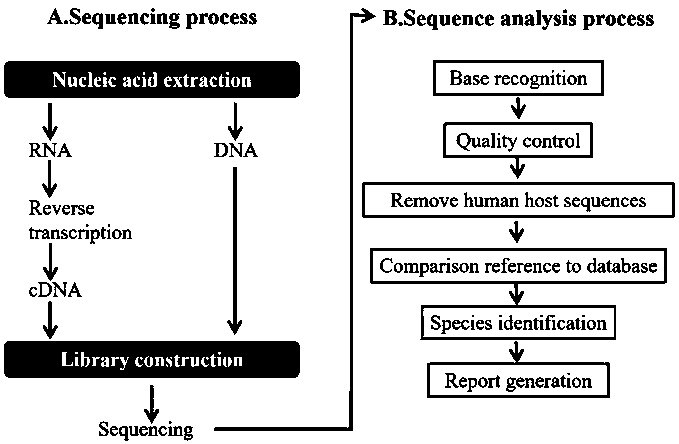
\includegraphics[width=0.6\textwidth]{img/analysis2}
    \caption{Phases comunes realizadas en un análisis de secuencias de ADN (Next-generation).}
    \label{fig:analysis}
\end{figure}
